% ============================================================
% Ejercicio 4
% ============================================================
\section{Ejercicio 4}

\begin{tcolorbox}[enunciado]
Para cada uno de los lenguajes del ejercicio 2:
\begin{itemize}[leftmargin=*]
    \item Define el lenguaje correspondiente al complemento.
    \item ¿A qué clase de complejidad pertenece el complemento?
    \item Da un ejemplar concreto que pertenezca al complemento.
\end{itemize}
\end{tcolorbox}

\begin{itemize}[leftmargin=*]
    \item \textbf{Problema DOM:}
    \subsection*{Solución}
    \subsubsection*{1. Definición del Lenguaje Complemento ($\overline{\text{DOM}}$)}

    El complemento del lenguaje se define como $\overline{\text{DOM}} = \Sigma^* \setminus \text{DOM}$:

    \[\overline{\text{DOM}} = \{ \langle G, K \rangle \mid G \text{ es una gráfica no dirigida que NO posee ningún conjunto dominante de } K \text{ nodos} \}\]

    Un ejemplar $(G, K)$ pertenece a $\overline{\text{DOM}}$ si y solo si la respuesta a la pregunta \textit{``¿Tiene $G$ un conjunto dominante de tamaño a lo más $K$?''} es \textbf{NO}.
    
    Es decir, $(G, K) \in \overline{\text{DOM}}$ si \textbf{para todo} subconjunto de vértices $C \subseteq V(G)$ de tamaño $|C| \le K$, existe al menos un vértice $v \in V(G) \setminus C$ que \textbf{no} es adyacente a ningún vértice de $C$.

    \subsubsection*{2. Clase de Complejidad a la que Pertenece $\overline{\text{DOM}}$}

    En el Ejercicio 2 se demostró que $\text{DOM} \in \mathbf{NP}$.
    Por definición de la clase complemento, si un lenguaje $L$ pertenece a \textbf{$\mathbf{NP}$}, su complemento $\overline{L}$ pertenece por definición a la clase \textbf{$\mathbf{coNP}$}:
    \[ \text{coNP} = \{ L \mid \overline{L} \in \mathbf{NP} \} \]
    Dado que $\text{DOM}$ es $\mathbf{NP}$, su complemento $\overline{\text{DOM}}$ es \textbf{$\mathbf{coNP}$}.

    \subsubsection*{3. Ejemplar Concreto que Pertenece a $\overline{\text{DOM}}$}
    \begin{figure}[H]
        \centering
        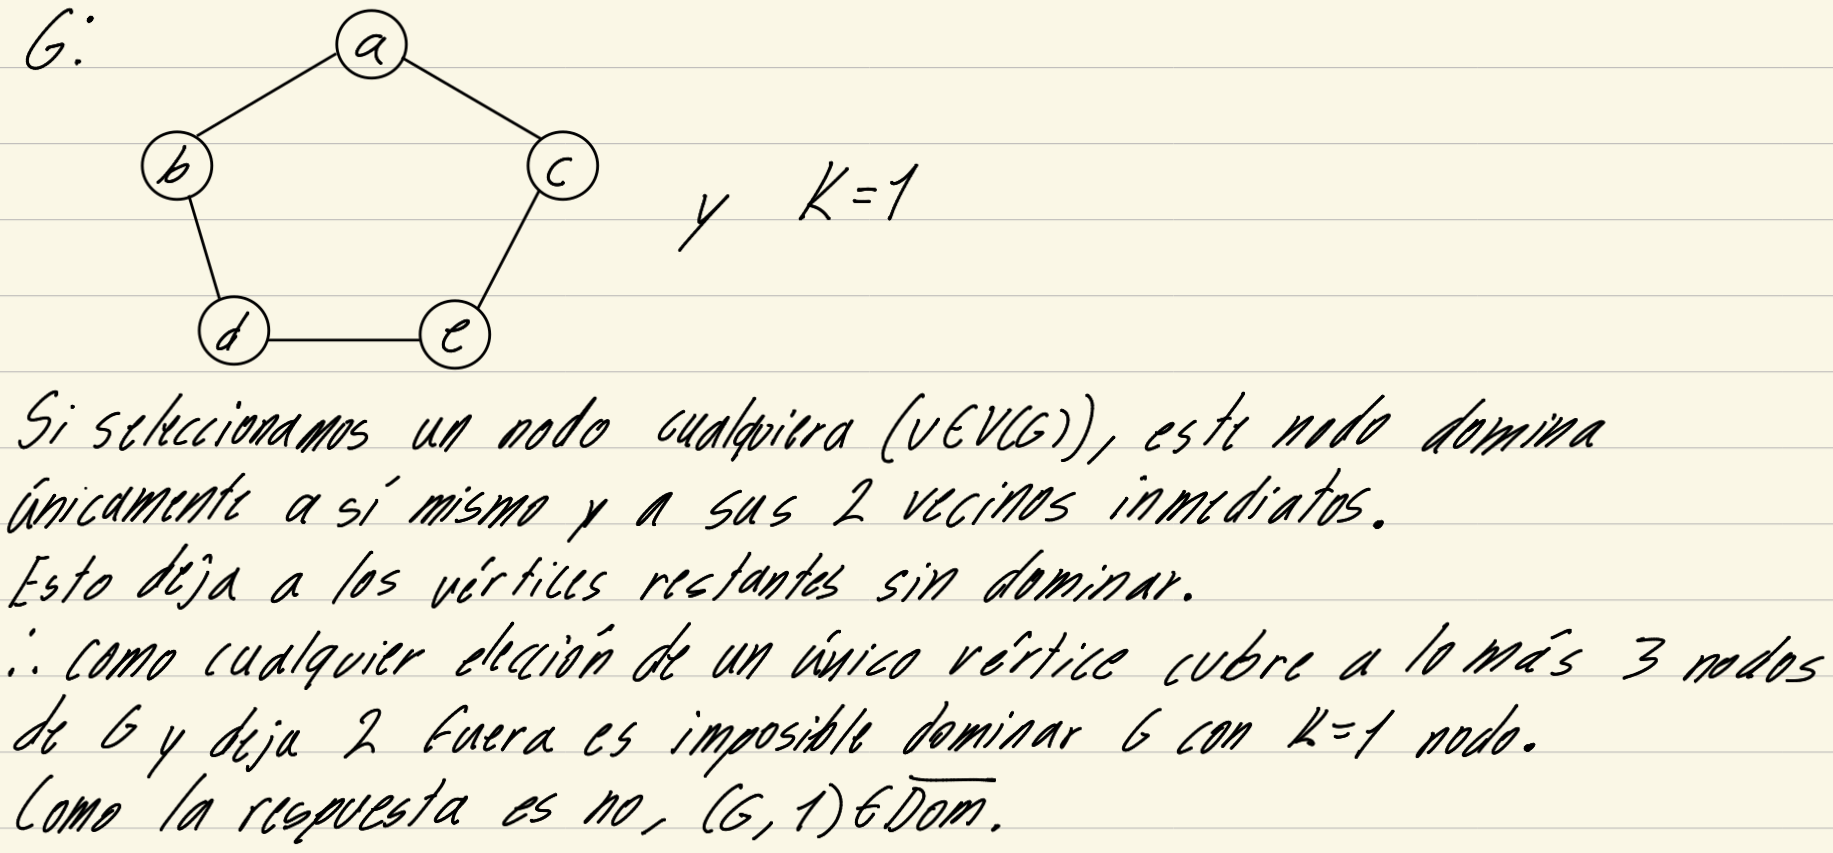
\includegraphics[width=0.8\linewidth]{imagenes/04_ejercicio/01_image.png}
    \end{figure}

    \vspace{0.5cm}
    \item \textbf{Problema L (No ciclos Eulerianos):}
    \subsection*{Solución}
    \subsubsection*{Definición del Lenguaje Complemento ($\overline{L}$)}
    El complemento del lenguaje se define como $\overline{L} = \Sigma^* \setminus L$:

    \[ \overline{L} = \{ \langle G \rangle \mid G \text{ es una gráfica no dirigida que SÍ contiene un ciclo Euleriano} \} \]

    \textbf{Por el Teorema de Euler:}\\
    Para las cadenas bien formadas que representan una gráfica conexa $G$, $\langle G \rangle \in \overline{L}$ si y solo si \textbf{todos y cada uno de los vértices de $G$ tienen grado par}.

    \subsubsection*{Clase de Complejidad a la que Pertenece $\overline{L}$}

    En el Ejercicio 2 demostramos que $L \in \mathbf{P}$ mediante un algoritmo determinista $M$ que calcula el grado de cada vértice y comprueba la conexidad mediante BFS/DFS en tiempo $O(|V| + |E|)$.

    Las clases de complejidad deterministas son \textbf{cerradas bajo la operación de complemento}:
    \[ \mathbf{P} = \text{co}\mathbf{P} \]

    Por lo tanto, si $L \in \mathbf{P}$ (y por inclusión, también pertenece a $\mathbf{NP}$ y $\mathbf{coNP}$), se concluye directamente que su complemento \textbf{$\overline{L} \in \mathbf{P}$}. El algoritmo determinista para $\overline{L}$ es idéntico al de $L$, invirtiendo únicamente los estados finales de aceptación y rechazo.

    \subsubsection*{Ejemplar Concreto que Pertenece a $\overline{L}$}
    \begin{figure}[H]
        \centering
        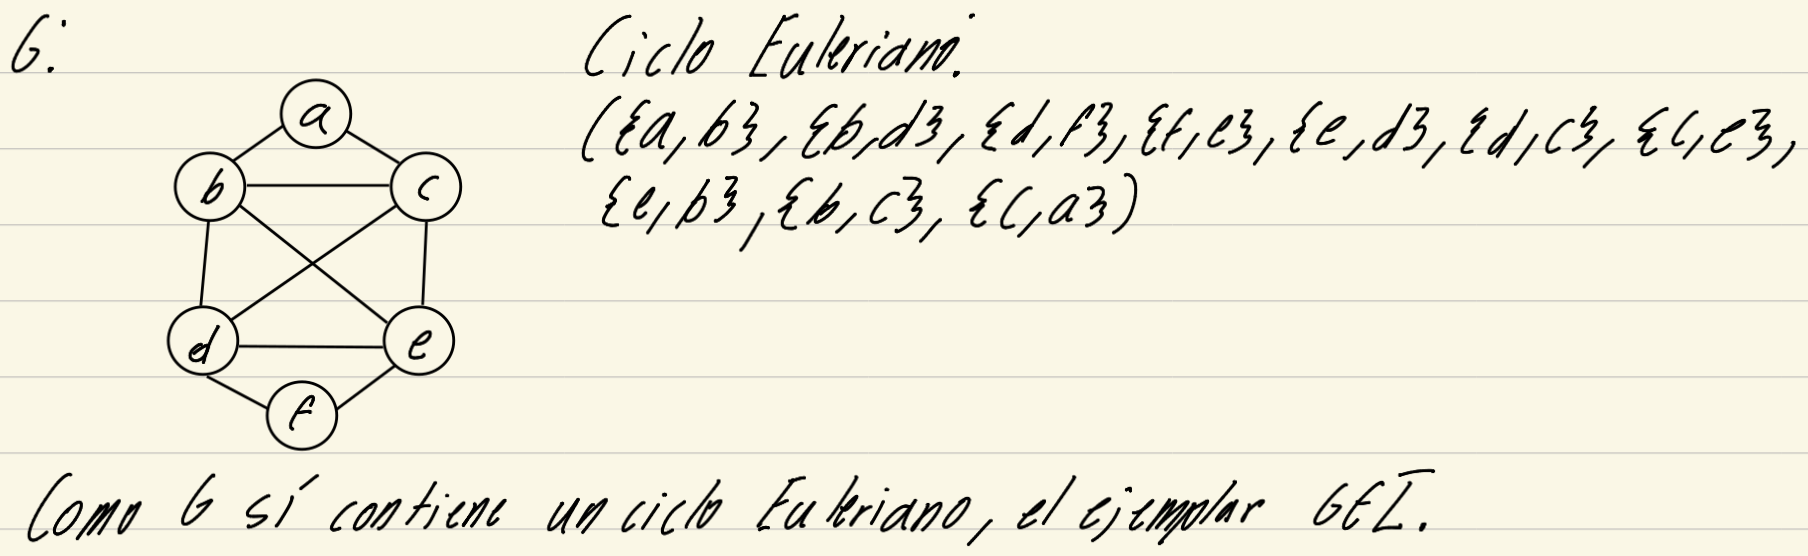
\includegraphics[width=0.8\linewidth]{imagenes/04_ejercicio/02_image.png}
    \end{figure}


    \vspace{0.5cm}
    \item \textbf{Problema HAM\_MOD:}
    \subsection*{Solución}
    \subsubsection*{Definición del Lenguaje Complemento ($\overline{\text{HAM\_MOD}}$)}

    El complemento del lenguaje es $\overline{\text{HAM\_MOD}} = \Sigma^* \setminus \text{HAM\_MOD}$. Aplicando la regla de la negación lógica (Leyes de De Morgan) a la conjunción original:
    \[ \neg \Big( (G_1 \in L_{\text{HAM}}) \land (G_2 \notin L_{\text{HAM}}) \Big) \iff (G_1 \notin L_{\text{HAM}}) \lor (G_2 \in L_{\text{HAM}}) \]

    Por lo tanto, formalmente se define como:
    \[ \overline{\text{HAM\_MOD}} = \{ \langle G_1, G_2 \rangle \mid G_1 \text{ NO tiene un ciclo Hamiltoniano } \mathbf{\lor} \ G_2 \text{ SÍ tiene un ciclo Hamiltoniano} \} \]

    Para que un ejemplar bien formado $\langle G_1, G_2 \rangle$ pertenezca al complemento $\overline{\text{HAM\_MOD}}$, la respuesta al problema original debe ser \textbf{NO}. Esto ocurre cuando se satisface \textbf{al menos una} de las siguientes dos situaciones:
    \begin{enumerate}[label=\arabic*., leftmargin=*]
        \item La primera gráfica $G_1$ carece de ciclo Hamiltoniano.
        \item La segunda gráfica $G_2$ sí posee un ciclo Hamiltoniano.
    \end{enumerate}

    \subsubsection*{Clase de Complejidad a la que Pertenece $\overline{\text{HAM\_MOD}}$}

    En el Ejercicio 2, dentro del marco del temario del curso, establecimos que $\text{HAM\_MOD} \in \mathbf{EXP}$ debido a que requiere decidir de manera exhaustiva dos propiedades intratables sobre dos gráficas distintas.

    Dado que las clases de tiempo determinista como $\mathbf{EXP}$ son \textbf{cerradas bajo complemento} ($\mathbf{EXP} = \text{coEXP}$), el complemento de cualquier lenguaje en $\mathbf{EXP}$ permanece dentro de la misma clase.

    Un algoritmo determinista de fuerza bruta puede verificar en tiempo exponencial si $G_1$ no tiene ciclo o si $G_2$ sí lo tiene, concluyendo la pertenencia a \textbf{$\mathbf{EXP}$}.

    \subsubsection*{Ejemplar Concreto que Pertenece a $\overline{\text{HAM\_MOD}}$}
    \begin{figure}[H]
        \centering
        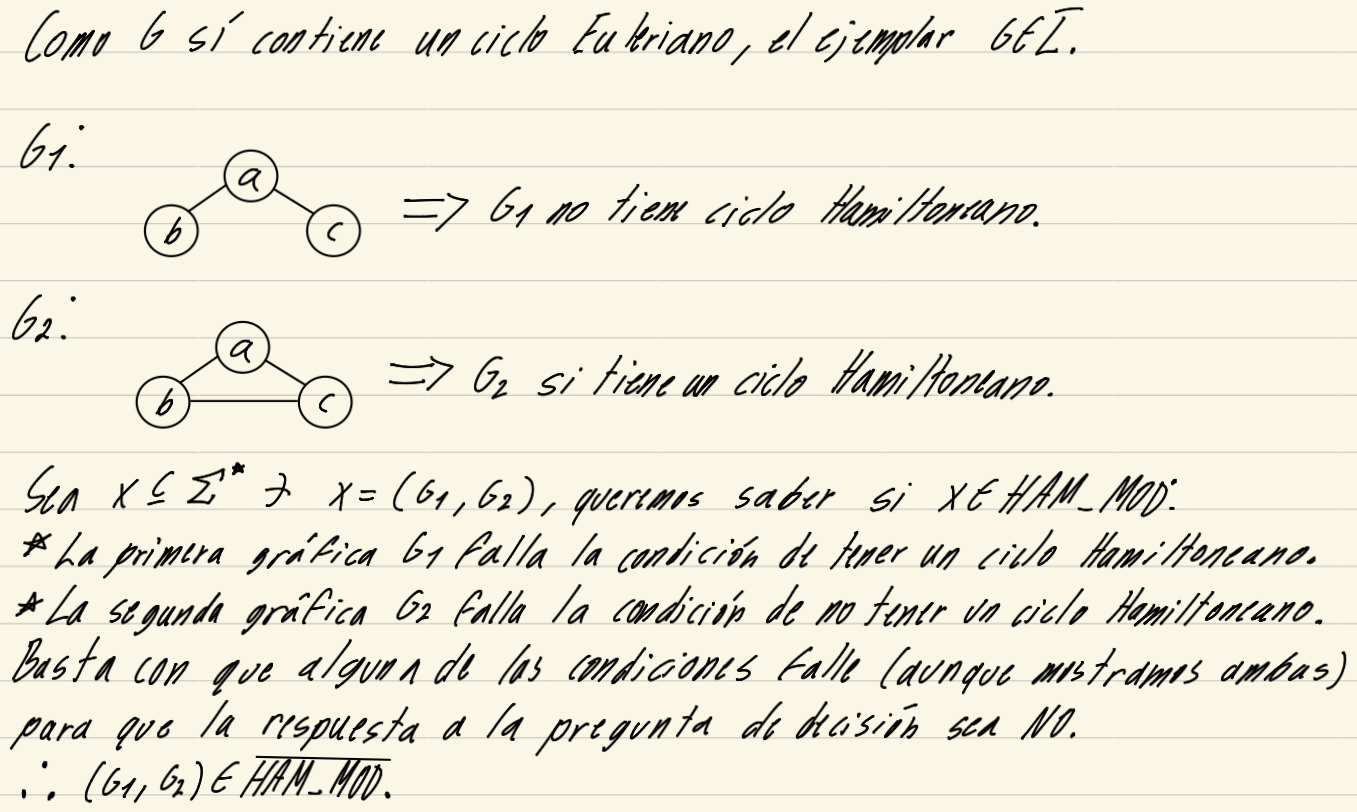
\includegraphics[width=0.8\linewidth]{imagenes/04_ejercicio/03_image.png}
    \end{figure}

    \vspace{0.5cm}
    \item \textbf{Problema CONECTIVIDAD:}
    \subsection*{Solución}
    \subsubsection*{Definición Formal del Lenguaje Complemento ($\overline{\text{CONECTIVIDAD}}$)}

    El complemento del lenguaje es $\overline{\text{CONECTIVIDAD}} = \Sigma^* \setminus \text{CONECTIVIDAD}$:
    \[ \overline{\text{CONECTIVIDAD}} = \{ \langle G \rangle \mid G \text{ es una gráfica no dirigida que NO es conexa (desconexa)} \} \]

    Una gráfica no dirigida bien formada $G = (V, E)$ pertenece a $\overline{\text{CONECTIVIDAD}}$ si es \textbf{desconexa}, lo cual significa que existen al menos dos vértices $u, v \in V$ entre los cuales no existe ningún camino en $G$ (es decir, la gráfica se compone de dos o más componentes conexas disjuntas).

    \subsubsection*{Clase de Complejidad a la que Pertenece ($\overline{\text{CONECTIVIDAD}}$)}

    En el Ejercicio 2 demostramos que $\text{CONECTIVIDAD} \in \mathbf{P}$ mediante un algoritmo determinista de Búsqueda en Anchura (BFS) o Profundidad (DFS) que explora la gráfica a partir de un nodo arbitrario $s$ en tiempo lineal $O(|V| + |E|)$.

    Las clases deterministas de complejidad de tiempo son \textbf{cerradas bajo la operación de complemento}:
    \[ \mathbf{P} = \text{co}\mathbf{P} \]

    Por lo tanto, si $\text{CONECTIVIDAD} \in \mathbf{P}$, se concluye directamente que su complemento \textbf{$\overline{\text{CONECTIVIDAD}} \in \mathbf{P}$} (y por inclusión, también pertenece a $\mathbf{NP}$ y $\mathbf{coNP}$).

    El algoritmo determinista para $\overline{\text{CONECTIVIDAD}}$ ejecuta la misma exploración (BFS/DFS):
    \begin{itemize}[leftmargin=*]
        \item Si la cantidad de nodos visitados desde $s$ es estrictamente menor que $|V|$, la máquina \textbf{Acepta} (devuelve \texttt{1}), confirmando que la gráfica es desconexa.
        \item Si la cantidad de nodos visitados es igual a $|V|$, la máquina \textbf{Rechaza} (devuelve \texttt{0}).
    \end{itemize}

    Como este procedimiento determinista toma tiempo $O(|V| + |E|)$, el problema se decide en tiempo polinomial.

    \subsubsection*{Ejemplar Concreto que Pertenece a $\overline{\text{CONECTIVIDAD}}$}
    \begin{figure}[H]
        \centering
        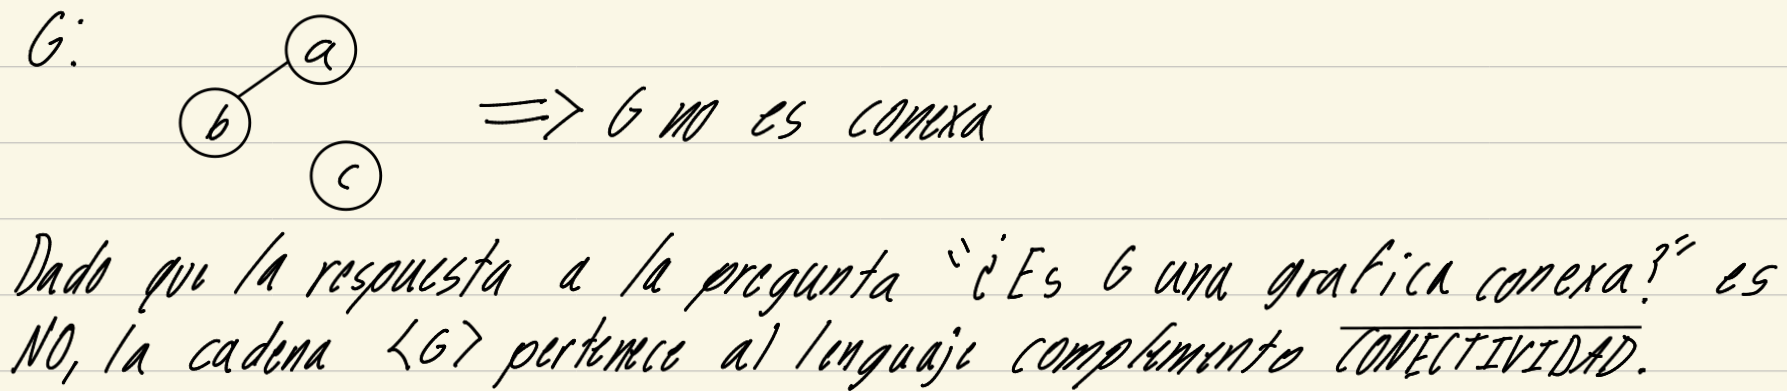
\includegraphics[width=0.8\linewidth]{imagenes/04_ejercicio/04_image.png}
    \end{figure}

    \vspace{0.5cm}
    \item \textbf{Problema CONJ\_INDEP (Opcional *):}
    \subsection*{Solución}
    % Escribe tu respuesta aquí

    \vspace{0.5cm}
    \item \textbf{Problema K-COLORACIÓN (Opcional *):}
    \subsection*{Solución}
    % Escribe tu respuesta aquí

    \vspace{0.5cm}
    \item \textbf{Problema EC-CUADRATICAS (Opcional *):}
    \subsection*{Solución}
    % Escribe tu respuesta aquí

\end{itemize}